\documentclass[conference]{IEEEtran}
\IEEEoverridecommandlockouts
% The preceding line is only needed to identify funding in the first footnote. If that is unneeded, please comment it out.
\usepackage{cite}
\usepackage{amsmath,amssymb,amsfonts}
\usepackage{algorithmic}
\usepackage{graphicx}
\usepackage{textcomp}
\usepackage{xcolor}
\usepackage{hyperref}
\def\BibTeX{{\rm B\kern-.05em{\sc i\kern-.025em b}\kern-.08em
    T\kern-.1667em\lower.7ex\hbox{E}\kern-.125emX}}
\begin{document}

\title{Attendance Tracking System\\}

\author{\IEEEauthorblockN {Stella Sravanthi Devarakonda}
\IEEEauthorblockA{\textit{Roll.No:  2019101101} \\
{IIITH}\\
{stella.sravanthi@students.iiit.ac.in}
}}


\maketitle

\begin{abstract}
Attendance the challenge which is seen in every institution.Even though our institution has bio-metric and attendance policy the real theme behind attending classes is sidetracking and ambiguity in planning the leaves by student is observed.In this paper, I'm going to present the software design of the Attendance Tracking System. This software designed for both students and professors so that both can have a track of attendance .  This involves mapping recognised face images to a list of students where face recognition technology here is black-box. The marking scheme is a very clear student is marked as absent or present based on the amount of time he spent in the respective class(or) lecture. I also described the software through detailed diagrams in section 3.
\end{abstract}

\begin{IEEEkeywords}
Bio-metric, Attendance policy, Attendance Tracking System
\end{IEEEkeywords}

\section{Introduction}
The motivation or problem statement is clear as the bio-metric attendance and attendance policy haven't fulfilled the importance of attending class and ambiguity in knowing the average class time by professors.therefore, we need highly appreciable software to store and manage the attendance of student and this is a major challenge. Issues with bio-metric attendance are immense raise in class strength just before class and immense downfall in the strength of the class after taking attendance which is not acceptable and beneficial to student and class environment. The attendance policy is not gaining its purpose because many come for attendance and then leave in the middle or whenever it is done. Having said the reasons we are now moving to appreciable software which is the application of face recognition and object detection technologies.This solution is well structured and tested consider this black-box. Now displaying or announcing the attendance immediately after the class  helps the professor to maintain student's interest and student to take leaves accordingly.

\section{Literature Review}

\subsection{Current Situation}
When professors look at student as a human on e can immediately recognises the presence and location. There has been so much research in developing the track of student's attendance system.We have various systems on using bio-metric or finger print technology, iris-based attendance system and face recognition attendance system also the Radio Frequency Identification based attendance system in different device based systems includes web, mobile.

\subsection{Methodology}
Unified Face recognition technology is widely used by many institutions.This technology mainly involves facial recognition which is done on measuring the facial features from a given respective image of student through ID authentication and tries to map these recognised images with student image database.Among different face recognition technologies from recent developments. We will discuss FaceNet and You Only Live Once (YOLO) approaches which are recognised as well structured but face challenges in implementation and recognition at respective scales.

\subsection{FaceNet}
This recent development is with very useful technology and easily implemented using standard techniques with FaceNet embedding as feature vectors.This also avoid the blockages layer and replaces that intermediate layer with deep convolutions network which is trained to directly optimize the embedding itself.Also the mapping here is directly to Euclidean space where  distances correspond to measure of face similarity without any doubt.
\subsection{YOLO (You Only Live Once)}
This development is to detect object and prior work on object detection re purposes classifiers to perform detection.Here the key technique or uniqueness is frame object detection which involves AI that is as regression problem to spatially separated bounding boxes and also associated class probabilities.We can guarantee about its optimisation because the whole detection pipeline is a single  network, and thus optimises end-to-end on detecting output directly.The advantage and disadvantage of this approach is YOLO's architecture is super fast and can maintain real-time speeds with high average precision and the drawback is making localization errors that is YOLO struggles to precisely localise some objects.But YOLO is learning and can learn pretty wide object representations.Methods like DPM,R-CNN are boosting up the training and learning process of YOLO this can effectively outputs detection and generalise the natural image or video frame to artwork(other domain).
\section{System Architecture}

Below are the images of two approcahes where the software developers can use them to get picturisation of whole software and can study the features deatliy.these models overview thr client about whole structure and concept we konow that sotware structure exemplifies the whole software content.Also this architecture is object-oriented and good enough to make changes or potential additions.\\[5mm]
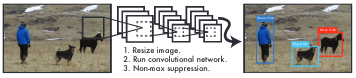
\includegraphics[width=\linewidth]{yolo.png}\\
\centerline{\caption{fig 1 . Yolo Detection System }}\\[5mm]
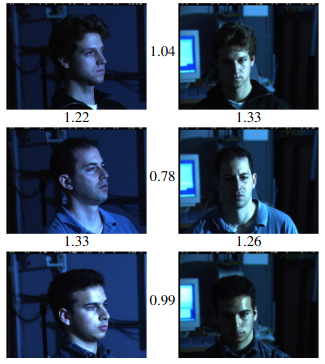
\includegraphics[width=\linewidth]{face.png}
\centerline{\caption{fig 2 . Illumination and Pose invariance }}
Here the face is recognised using camera and calculation of time spent in class room is specified in specifications and classified.
\subsection{Specification}\label{AA}
Using camera face recognition is happened and this is placed near door step of class room , this software mainly calculates the time spent by respective student on counting the number of in and outs of the student and store the time.Also this can be web based system since it friendly to use and no need of extra hardware and it has efficient techniques to store and update the student attendance and report in the Web  Site. \\[9mm]
One can classify the requirements of this software into Functional and Non-functional Requirements.\\[3mm]
Functional Requirements:\\[2mm] Both faculty and student able to login and have separate pages.Admin exists to manage the entire system.\\[2mm]
While registering student should be able to provide his/her face image along with basic details like name and roll number.\\[2mm]
Student has a dashboard to report/take a leave due to any valid reason which involves approval of administration.\\[5mm]
Non-functional Requirements:\\[2mm]
Here the website can be utilised from any type of devices.System's accuracy,dependability, durability are prime requirements of any software system.\\[1mm]
Thus here due to usage of software in  any device this meets compatibility and real-time computation also the design is unambiguously easy to use by both users.\\[2mm]
\subsection{Design and system Diagram}
\\[3mm]
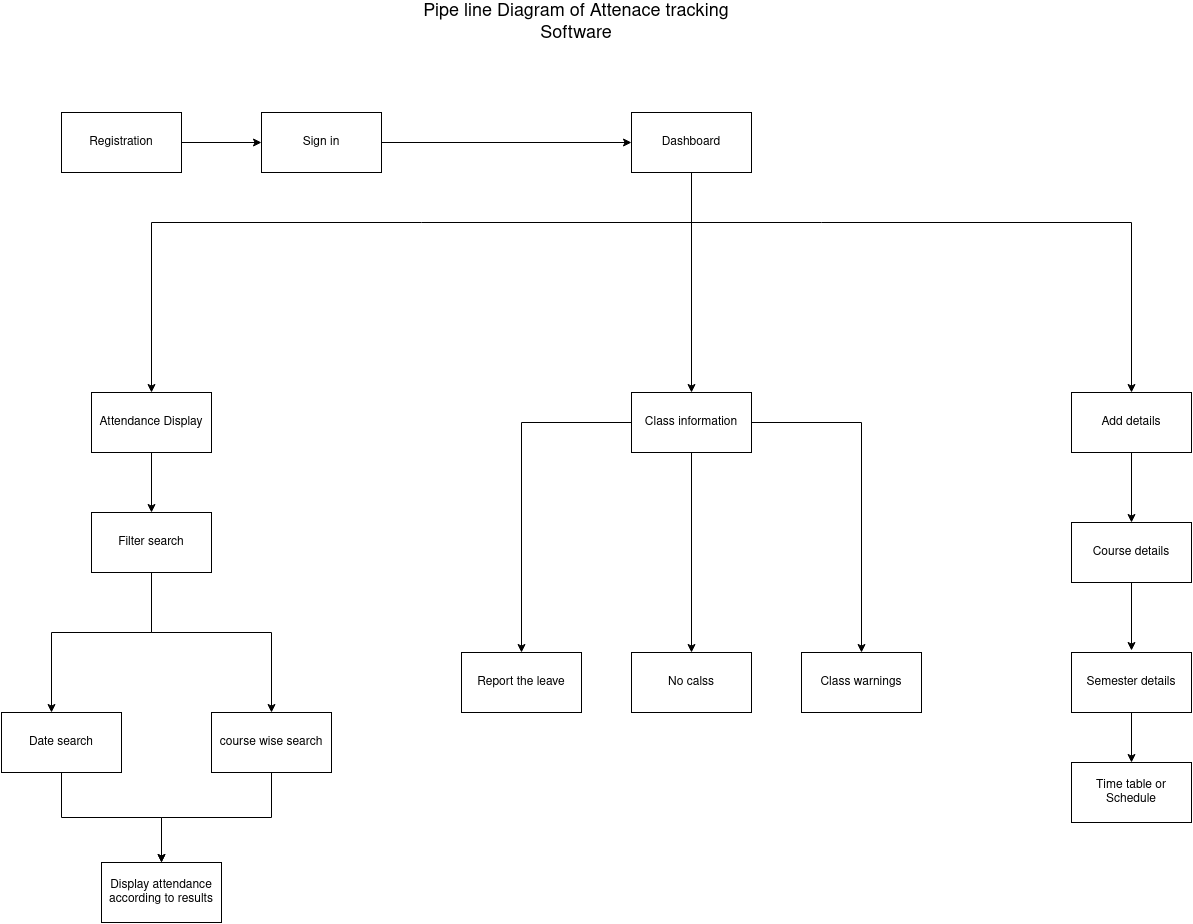
\includegraphics[width=\linewidth]{pieline.png}\\
Application design of this Attendance Tracking system and each user has following duties or options to do in the website.\\[1mm]
First and foremost . Since we are developing this software for faculty's happiness and also to  view the attendance by individual student.\\
\textbf{Professor or Faculty user:}\\[2mm]
Professor register in this software using basic details like name, course id.\\
Professor can login into this software.\\
Professor can add the schedule of the course.
Professor can able to cancel the class with reasonable causes and announcement.\\
Professor can  view the average attendance of student after every class.\\[3mm]
\textbf{Student user:}\\[2mm]
Student can register to this system using face feature and by giving formal details of their name,roll number and email id .\\[1mm]
Student login into system and see the list of courses.\\[1mm]
Student and view his/her attendance after every class .\\[1mm]
Student has dashboard to view the attendance courses wise.\\[1mm]
Student  get warnings  for  the  specified period.\\[1mm]
Also student can able to apply for leave with any valid reasons.\\[2mm]
\textbf{Admin user :}\\[2mm]
Admin user can manage the database and  has  all  the privileges  over  this software system  to  control  everything  within the system.\\[1mm]
Admin user adds the courses of respective student by knowing his/her details.\\[2mm]
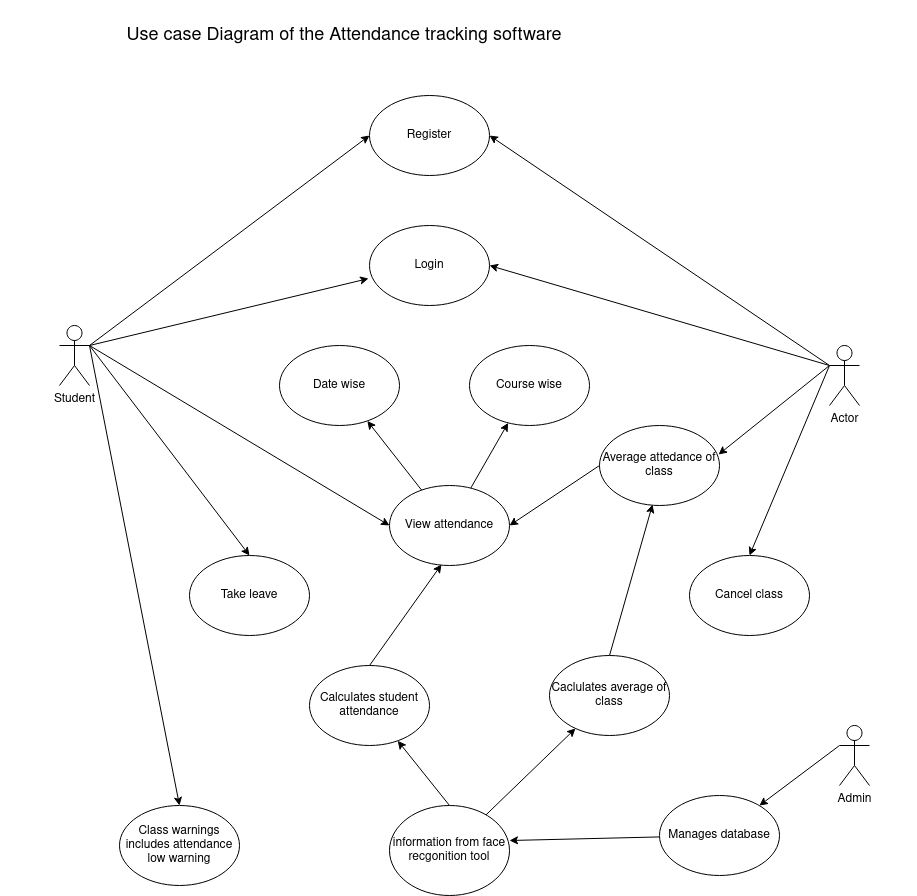
\includegraphics[width=\linewidth]{use case.png}\\

\textbf{\subsection{Scheme or backend  work}}
Student is marked as absent if the amount of time student been in class room for the respective course is less than half of the lecture duration.\\
Faculty can view the average class timings of the course and improve their teaching methods to develop the student's interest.\\[2mm]
Thus on stating the application design the software system has two main sites public,private where the public involves the logins by anyone who has registered and private site is for admin user who can control everything and this is known as backend too.  \\[1mm]
Admin manages to store the data right from beginning whenever the user is registered stored as unique id and when the attendance is marked software updates the calculated attendance in respective student's portal and also contributes to average class time in faculty portal.
 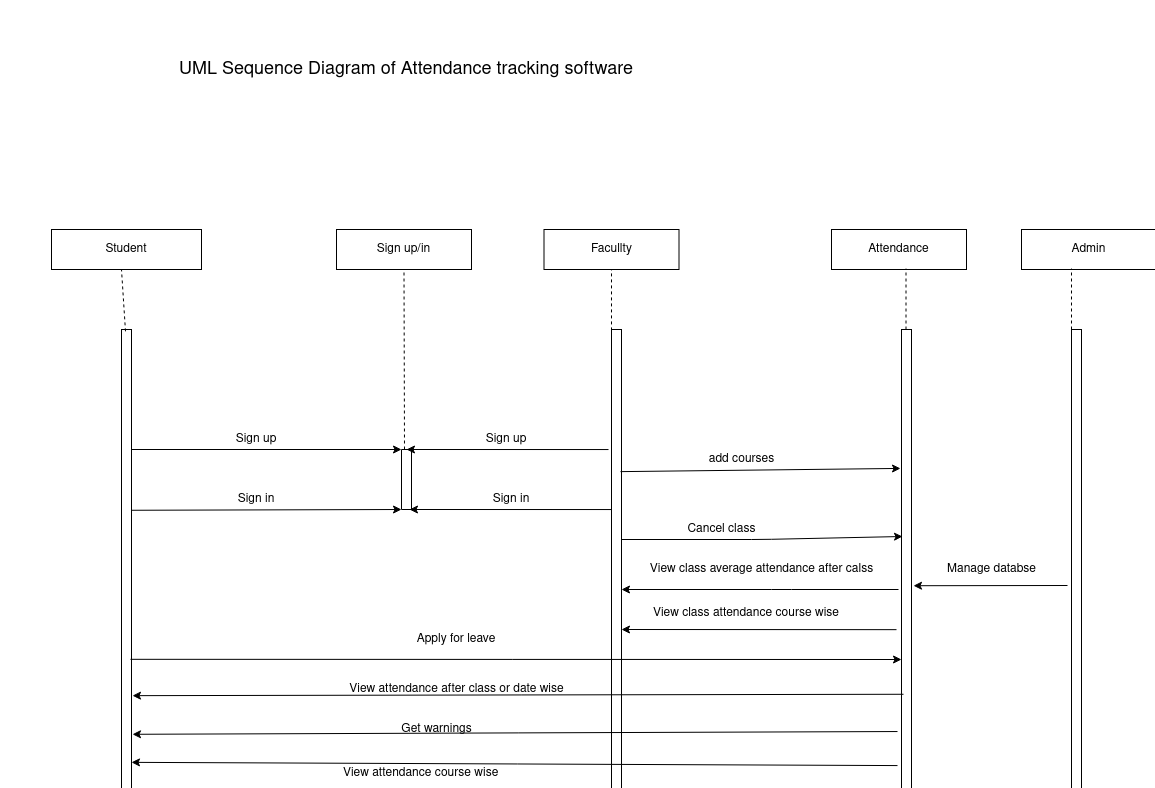
\includegraphics[width=\linewidth]{seq.png}\\
Check the PipeLine,Usecase and UML diagrams clearly
\href{https://drive.google.com/file/d/1psgtDoe6vJ8_oiQ68vjRNNF3smwc8VLt/view?usp=sharing}{here}.
\section{Conclusion and future work}
Attendance  management  is important to  all  educational  institutions.Specifically the attendance tracking system is badly needed in our institution as it can reduce the burden or dissatisfaction of faculty and helps students to  manage leaves  by keeping track of their attendance and faculty to  maximize  their  performance. In this paper, we show the architecture of attendance tracking  software. The design of the system is also discussed such as revolutionary face recognition technologies. We assume that putting these ideas into practise in future would benefit students and faculty in a variety of ways.
\section{REferences}
[1]FaceNet: A Unified Embedding for Face Recognition and Clustering\\
[2] You Only Look Once: Unified, Real-Time Object Detection.
\end{document}
